\begin{frame}{On est perdu!}
  \begin{columns}
    \column{0.4\textwidth}
      \begin{center}
        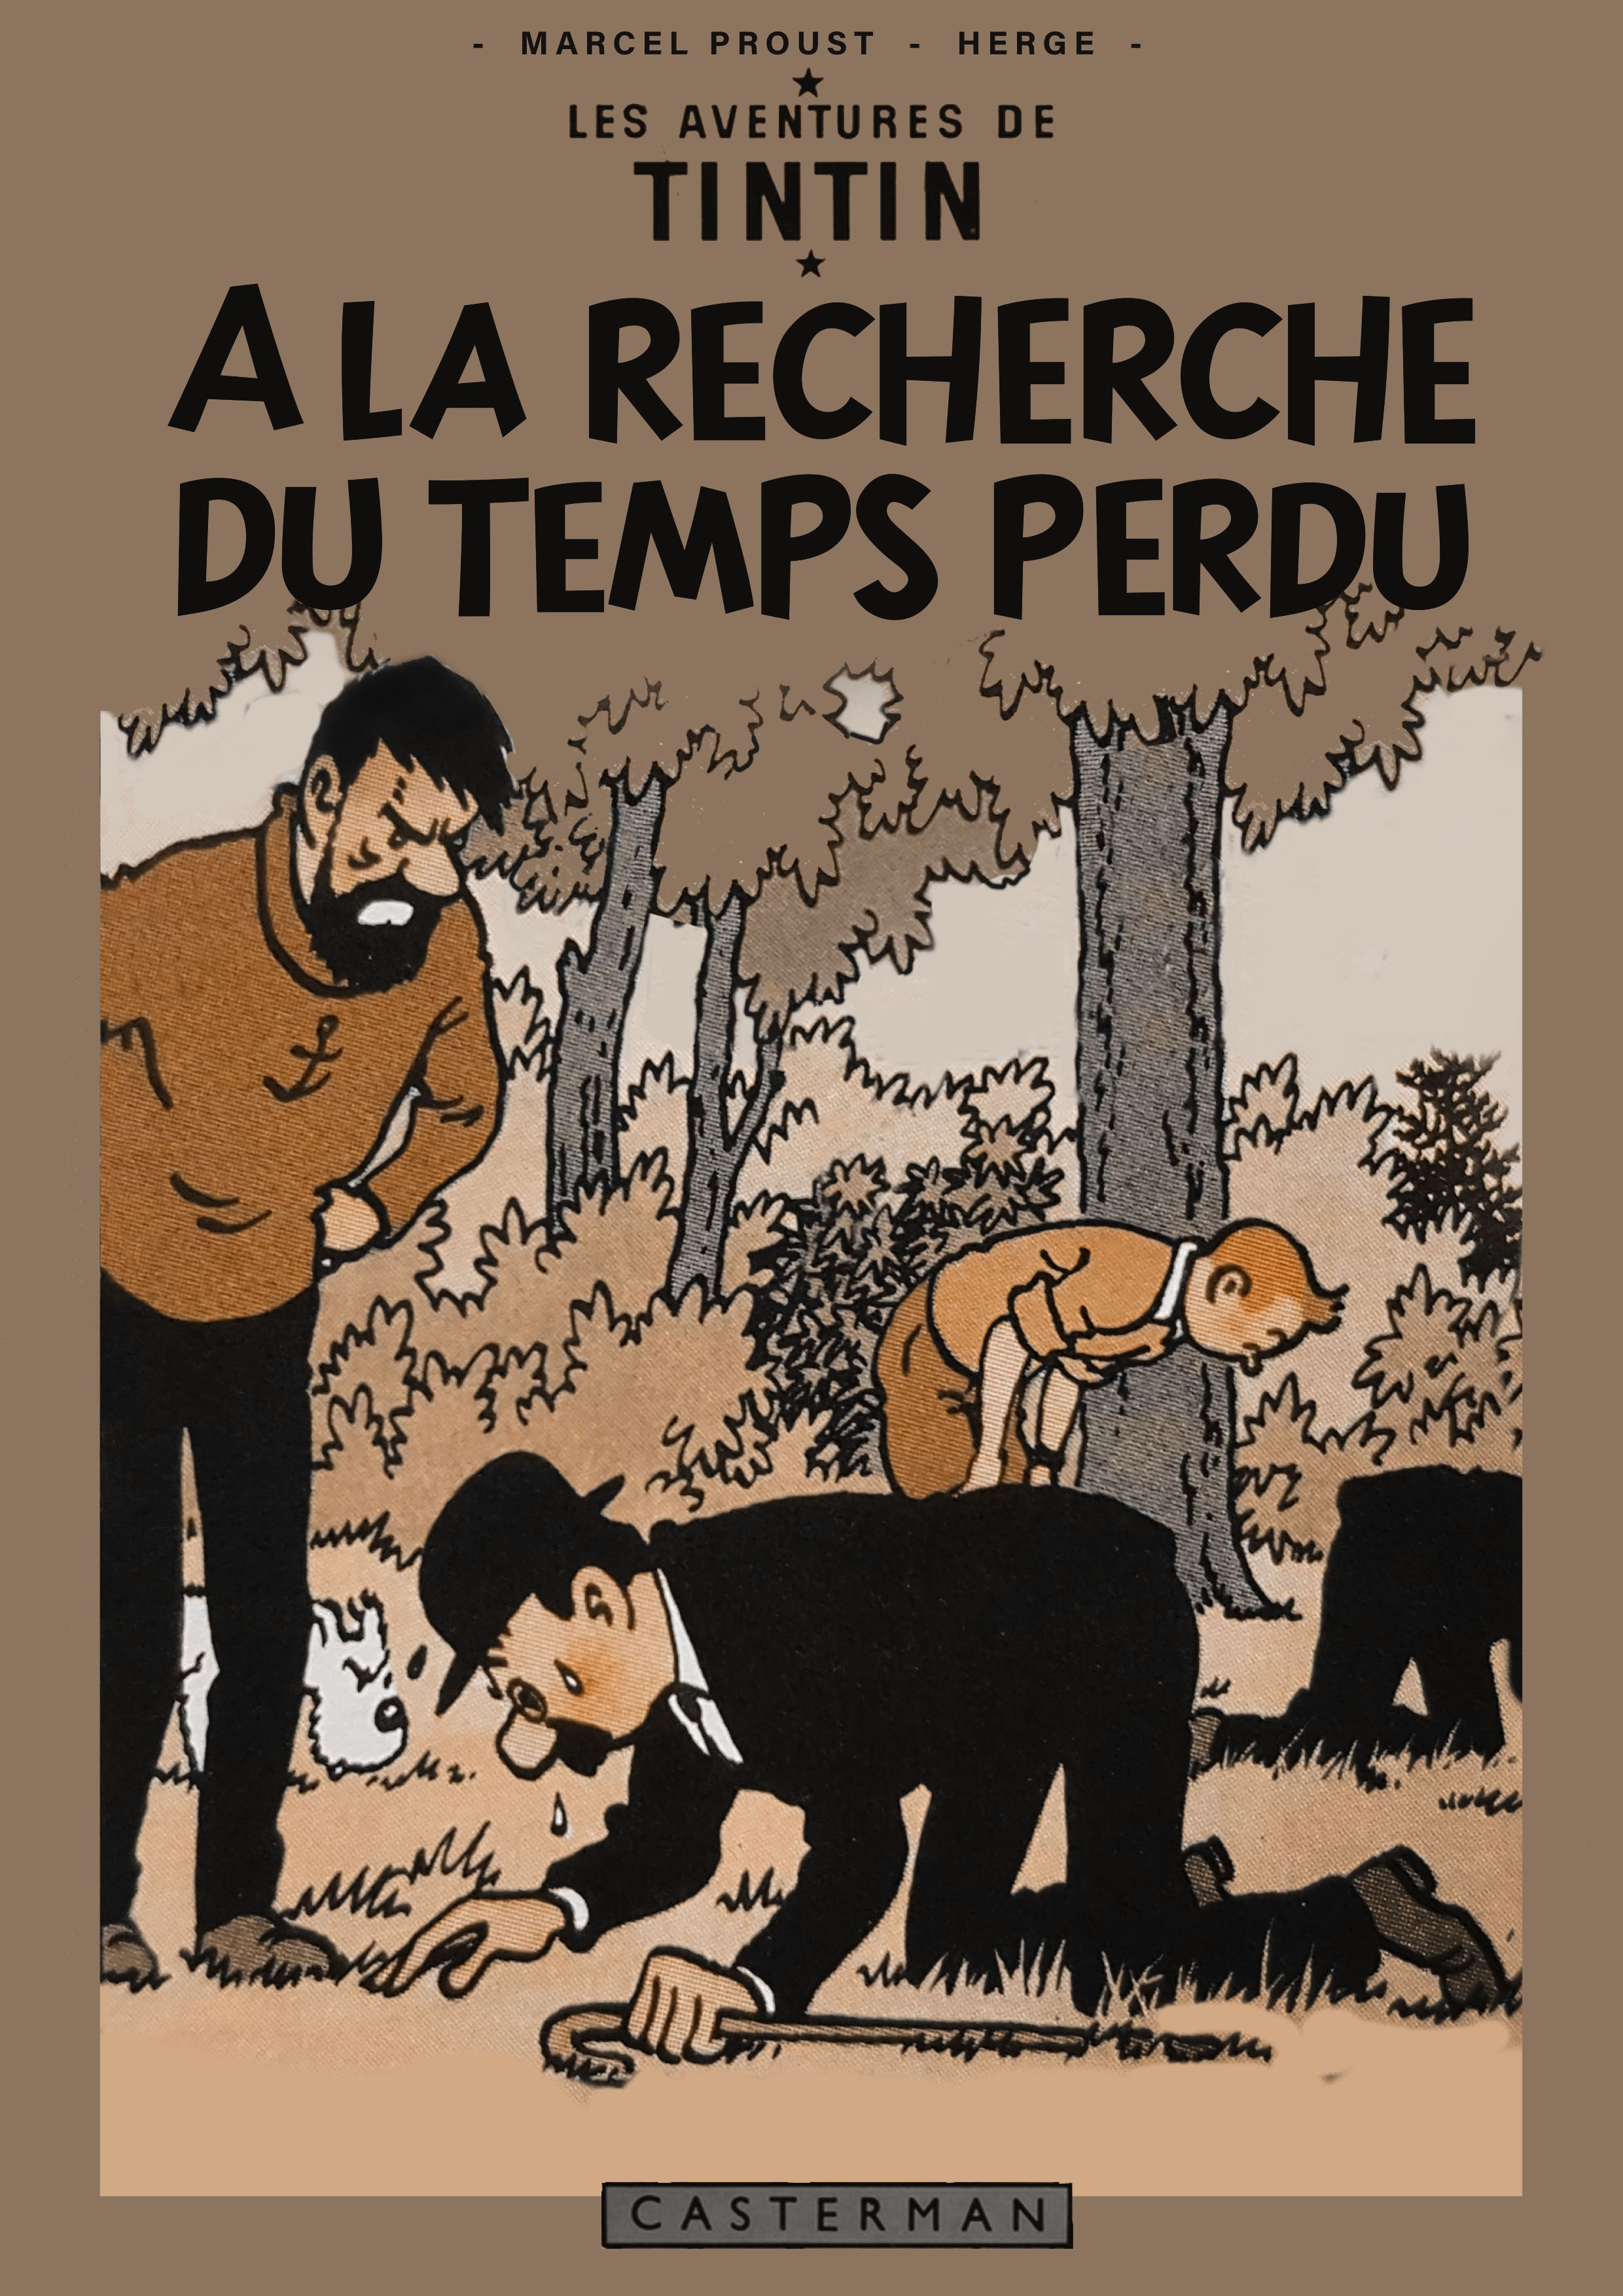
\includegraphics[scale=0.045]{tintin_temps_perdu.jpg}
      \end{center}
    \column{0.6\textwidth}
      Est-ce que \alert{tu te perds} quelquefois?
      Où est-ce que \alert{tu te trouves} à ces moments? 
      Est-ce que \alert{tu visites} un endroit en particulier lorsque cela se passe?
      Qu'est-ce que \alert{tu cherches} lorsque tu te perds?
      Discutes-en en groupes.
      \begin{description}
        \item[] \textbf{Modèle:}
        \item[E1:] Moi, \alert{je me perds} quelquefois quand \alert{je cherche} une nouvelle classe, surtout dans le bâtiment de journalisme. \alert{Je me trouve} tout le temps sur le mauvais étage!
      \end{description}
  \end{columns}
\end{frame}